\documentclass[a4paper,10pt]{article}
\usepackage[utf8]{inputenc}
\usepackage{fullpage}
\usepackage{color}
\usepackage{authblk}
\usepackage{listings}
\usepackage{graphicx}
\usepackage{subfigure}

%PREPRINT/MANUSCRIPT OPTIONS
\usepackage{setspace}
\usepackage{lineno}
\linenumbers
\doublespacing

\definecolor{codegreen}{rgb}{0,0.6,0}
\definecolor{codegray}{rgb}{0.5,0.5,0.5}
\definecolor{codepurple}{rgb}{0.58,0,0.82}
\definecolor{backcolour}{rgb}{0.95,0.95,0.92}
 

\title{Gsmodutils: A python based framework for test driven genome scale metabolic model development}
\author[1]{James Gilbert}
\author[1]{Nicole Pearcy}
\author[2]{Jamie Twycross}
\author[3]{John King}
\author[1]{Nigel Minton}
\affil[1]{Synthetic Biology Research Centre, University of Nottingham, Nottingham, NG7 2RD, United Kingdom}
\affil[2]{Intelligent Modelling and Analysis group, School of Computer Science, University of Nottingham, Nottingham, NG7 2RD, United Kingdom}
\affil[3]{School of Mathematical Sciences, University of Nottingham, Nottingham, NG7 2RD, United Kingdom}

\begin{document}

\maketitle

\begin{abstract}
\textbf{Motivation:} Genome scale metabolic models are increasingly important for systems biology and metabolic engineering research as they are capable of simulating complex steady state phenotypic behaviour.
Constraints based models of this form can include thousands of reactions and metabolites, with many crucial pathways that only become activated in specific simulation settings.
However, despite their widespread use, power and the availability of tools to aid with the construction and analysis of large scale models little methodology is suggested for the management of continually curated large scale models.
This is quickly becoming an issue for industrial systems and synthetic biotechnology applications, which require good quality reusable models integral to the design, build and test cycle.
\\
\textbf{Results:} Taking advantage of python and cobrapy integration, we have developed the \textit{gsmodutils} modelling framework.
As a fully documented python API and series of command line utilities, gsmodutils places an emphasis on test driven design of models through easy to write test cases in json or python.
Crucially, different substrate conditions are configurable allowing users to examine how different designs or curation impact a wide range of system behaviours, hopefully, minimising error between model versions.
Furthermore, a core feature of the software is to allow users to easily create shareable, self contained, docker images that can be run in cross platform environments.\\
\textbf{Availability:} The software framework described within this paper is open source and freely available from http://github.com/gsmodutils \\
\textbf{Contact:}{james.gilbert@nottingham.ac.uk}
\end{abstract}


\section{Introduction}
Stoichiometric constraints based modelling for biological systems has been a mainstay of systems biology for several decades \cite{fell1986fat, varma1994stoichiometric}.
Given its flexibility, low barrier to entry and requirement only on minimal knowledge regarding the stoichiometry of metabolic networks this structural approach has become an extremely popular method for modelling steady state behaviour of large, biochemical networks \cite{kauffman2003advances}.
Such large scale reconstructions are often refereed to as genome scale models (GSMs), as the processes is significantly aided through the advent of relatively inexpensive genome sequencing \cite{o2015using, land2015insights}.

The reconstruction of GSMs is an arduous process that follows a complex protocol to ensure model validity \cite{thiele2010protocol}.
Whilst many popular automated methods exists to construct GSMs from reference genomes \cite{henry2010high, poolman2006scrumpy}, there is a still a significant amount of manual curation.
However, treating the creation of models as an isolated ``one-off'' event ignores the significant amount of curation that is required for applications such as biotechnology.

As a consequence, a significant amount of work has gone into the management of genome scale models.
The BiGG models database \cite{king2015bigg}, for example, exists to provide a standardised repository of validated models that can be shared and reused.
However, little focus is placed upon the collaborative design aspect of such models with few mechanisms existing to store the \textit{model delta} based tools provided in our software.
Similarly, the MetaNetX \cite{moretti2016metanetx} system exists to provide a standardised namespace and toolchain for GSM analysis.
However, such tools often make it difficult to understand the design decisions made by the initial model authors.

Furthermore, as with many areas of bioinformatic study the proliferation of available computational tools has become somewhat vast.
This covers huge variety of software platforms including the COBRA toolbox in Matlab \cite{schellenberger2011quantitative}, ScrumPy and CobraPy in Python \cite{poolman2006scrumpy, ebrahim2013cobrapy} with additional tools and libraries such as cameo \cite{cardoso2017cameo}, OptFlux in Java \cite{rocha2010optflux}, SurreyFBA \cite{gevorgyan2010surreyfba}.
Whilst most of these tools are Open Source and follow standards, such as SBML \cite{finney2003systems}, there are often few options that make analysis easy to replicate.

The archetype design, build and test cycle of synthetic biology heavily relies on the usage of bioinformatics software and modelling to improve the production of natural products \cite{carbonell2016bioinformatics}.
In order to speed up the use of bioinformatics tools to produce high value platform chemicals, genome scale models are often used to discover methods for process optimisation \textit{in silico}.

For example, many tools such as RetroPath \cite{carbonell2013retropath}, XTMS \cite{carbonell2014xtms} and GEM-Path \cite{campodonico2014generation} suggest thousands of potential hetrologous pathways as well as providing predictions for flux distributions.
Many of these tools significantly increase the value of genome scale models, for example by coupling commodity production to an organism's growth \cite{feist2010model}.
These tools all suggest major changes to wild-type strains must be tracked and compared to allow models to remain relevant.
In effect, mechanisms are required to related modified models to modified test and production strains.

Similarly, many conventional applications of genome scale models in systems biology have often suffered from unnecessary replication of work due to a lack of standards.
For example, there are now many independently developed models of \textit{Clostridium acetobutylicum} \cite{lee2008genome, senger2008genome, mcanulty2012genome, dash2014capturing, yoo2015quantitative}, an organism used in the production of solvents for over a century.
These models all exist to solve similar biological problems some being updates to the inital base models. 
However, there has been disagreement over fundamental biochemical properties of these anaerobic organisms, notably with the focus on redox balancing \cite{dash2014capturing}.
Indeed, such models also include updates based on improved genome annotations and the inclusion of fluxomic, transcriptomic and metabolomic characterisations \cite{yoo2015quantitative}.

Many of the results presented in original sources are difficult to compare due to a lack of standardisation of reference identifiers for reaction names.
Where models are shared they are often in non-standard spreadsheet formats, rather than SBML models.
Indeed, even in the case of valid SBML models being made available at the time of publication few details are given as to how to run such models.

% Perhaps more worryingly, from an industrial perspective, is that the use of models in bioproduction has not escaped regulatory notice \cite{}.
Furthermore, as models are often used to explain issues with online production and facilitate the optimisation of bioprocessing, it stands to reason that model correctness should attract oversight.
Consequently, methods are needed to ensure that the models themselves are tightly version controlled.
In this paper, we argue for the use of a form of \textit{test driven} model of development, a conceptual approach borrowed from software engineering.
Given the availability of widespread open source virtualisation tools that allow the standardisation of platforms \cite{merkel2014docker}, modellers have the opportunity to share highly reproducible research \cite{chamberlain2014using}.

In this paper we present a software framework geared toward \textit{test driven} genome scale model development, a concept that is taken directly from good software development practices.
By this we mean the notion that, as a model is curated to represent biological phenomena, much of the validation can be turned into specific test cases that can be repeated between model versions.
We provide an example test case for \textit{C. acetobutylicum} an organism that has had considerable focus in terms of genome scale models and how a working methodology using the software presented here can reduce repetition of work and improve the reproducibility of results.
This article aims to summarise the main objectives of the gsmodutils software and we refer the reader to the software user guide for a more detailed exploration features.

\section{Improving the design phase of industrial biotechnology}

The design phase of industrial synthetic biotechnology, due to historical and regulatory convention, often follows a waterfall model for development of genome scale models.
This is borne out of a number significant constraints in the development of genome scale models.
The waterfall approach for model is characterised in Figure \ref{fig:methodology_approaches} where requirements for a model are captured at an early stage and are hard to refine during the production process.

In contrast, an \textit{agile} methodology for the development of models places the focus on adapting work to new requirements \cite{martin2002agile}.
Such an approach best fits genome scale models because they are rarely created to investigate individual processes and, instead, capture the complexity of large systems.
Constraints based models are intrinsically related to available genome annotations.
Such annotations rely heavily on automated matches to related species, with the characterisations of individual genes often being left to a few of critical interest \cite{seemann2014prokka}.
This modelling formation costs an in depth understanding of dynamic behaviour. 
However, capturing steady state phenomena still provides a good understanding of systemic properties \cite{o2015using}.

As such approaches often leave models with missing reactions, incorrect gene-reaction rules \cite{thiele2010protocol} or with pathways based on gap filling methods that add reactions that may not be present within the organism \cite{benedict2014likelihood}.
When attempting to understand specific natural phenomena, genome annotations are frequently updated and models are often corrected in an \textit{ad hoc} manner.

\begin{figure}[ht]
\includegraphics[width=\textwidth]{Waterfall.png}
\caption{Conventional waterfall methodology for model development.
Each process is considered to be an isolated aspect of model development.}
\label{fig:methodology_approaches}
\end{figure}

Therefore, models undergo significant manual annotation - a process which naturally leads to errors.
In this work we advocate a test driven approach to model development highlighted in Figure \ref{fig:test_driven}.
Here, the model is changed to achieve core research goals that are dynamic in response to the changes of a project.
In order to meet this objective, validation criteria for a model such as growth conditions or the impact of gene knock outs, should be formally set.
When a model is changed, all such validation criteria should be retested to ensure that models do not regress to previous states.

\begin{figure}[ht]
\centering
\includegraphics[width=0.5\textwidth]{Testdriven.png}
\caption{Workflow for model development proposed for gsmodutils.
The objective of this approach is to simultaneously capture research questions, model validation criteria and minimise the impact of changes on previously completed models.
}
\label{fig:test_driven}
\end{figure}

We feel that while many of the current software tools for genome scale models do an excellent job of facilitating answers to crucial research and design questions.
However, their is a major gap in terms of the reliability and re-usability of models due to a lack of standardisation and software tools to aid such processes.
The following sections provide an overview of the gsmodutils software framework.
Gsmodutils aims to provide a basis for test driven, version controlled agile model development.
All software is open source and is designed to be interoperable with platforms widely used in the domain of constraints based modelling.

\section{Software}

\subsection{Outline and features}
Test driven development is driven by the idea of clearly defined test cases written before significant changes are made to any underlying architecture.
In the case of genome scale models, errors occur as a product of human curation to better represent newly discovered aspects of metabolism.

By automatically integrating the COBRAPy \cite{ebrahim2013cobrapy} users can easily write convenient test cases following examples given in the user guide.
A standard test case, ensuring that a given model grows on media is given in Box \ref{fig:test_case}.
When a new model repository is created with the gsmodutils tool, a number of pre-written test cases are automatically added to a file.
However, we stress that the vast majority of individual use cases for a model must be specific to a given biological problem.

The software provides a number of features such as import an export of models in different formats and the generation of test reports through use of the command line. 
The use of flat files for easy integration with version control software such as git and mercurial.

In addition, projects are easy to export using portable standardised docker images \cite{merkel2014docker}. 
The idea being to allow users to share models as quickly and easily as possible without concern for custom system configurations.


\begin{figure}[ht]

\lstset{language=Python}   
\begin{lstlisting}
def test_func(model, project, log):
    status = model.solver.optimize()
    log.assertion(status == 'optimal',
                  ``Works'', # Success message
		  ``Does not work'', # Failure message
                  ``Test description'')
\end{lstlisting}
\label{fig:test_case} 
\caption{An example gsmodutils test case written in python}
\end{figure}

\subsection{Strain designs}
A core aspect behind the implementation of gsmodutils is the concept of a \textit{design}, this encompasses a simple set of changes to a ``wild-type'' model that are required for analysis.
For example a mutant strain that has undergone several gene deletions is not sufficiently different from the original wild-type to merit having its own genome scale model.
However, it is often the case that such deletions are of scientific or industrial interest and, as such, the strain will be used in future work.
Consequently, such designs are hereditary in nature.
By taking the delta between the constraints applied to an initial model and subsequent modifications, gsmodutils allows users to easily reuse and export models with this design.
As designs inherit from a base model, future curation to a wild type model will automatically be included in the designs.
Similarly, designs are self contained and will not interfere with one another allowing a form of project management.
Figure \ref{fig:strain_hered}

\begin{figure}
  \includegraphics[width=\textwidth]{inheritence.png}
  \label{fig:strain_hered}
  \caption{Examples of gsmodutils design inheritance.
  Each design stores the delta between the wild-type base model, any parents and the changes to constraints the design contains.
  In the example presented above a hetrologous production pathway is combined with a reusable set of knock-outs.
  In practice, ideally, these designs should relate to real constructs and strains evaluated by wet lab biologists.
  }
\end{figure}

\subsection{Development workflow}
In this section we propose a method for the development of genome scale models that integrates gsmodutils with version control systems.
Figure \ref{fig:test_case} highlights the notion of test cases, taken from test driven development.
The outlined workflow is that the user writes a formal test case for some modelling goal, perhaps driven by captured experimental data, that fits a specific form of validation criteria.
We note that, in principle, this test case should be written \textit{a priori} of changes to a model.

\section{Example usage Clostridium acetobutylicum models}
\subsection{Scientific background}
\textit{C. acetobutylicum} ATCC 824 is a widely researched organism that has found use in the production of solvents for decades.
More recently, \textit{C. acetobutylicum} has been applied for the production of alcohols such as ethanol and n-butanols.
The industrial relevance and strong background of experimental data has led to the application of many genome scale models \cite{}.
Whilst increasingly informative when combined with experimental data, the history of the management of models for \textit{C. acetobutylicum} tells a different story.

Initially, two rival models were published containing a similar number of genes \cite{lee2008genome, senger2008genome}.
% \textbf{TODO: describe in more detail}.
%Discuss limitations of rival models
This led to the further development of subsequent models, iCaC 490 \cite{mcanulty2012genome} and an automatically generated model from  the Model SEED  pipeline \cite{}.

In this example we focus on the more recent contributions of iCac802 \cite{dash2014capturing} and iCac967 \cite{yoo2015quantitative}.
iCac802 combines a significantly updated set of annotations from previously curated model versions, an improved TCA cycle, full proton balancing in reactions and reactions for more complete coverage of hexadecanoyl-acp, hexadecanoyl-CoA, crotonyl-CoA pathways as well as pathways for the uptake and biosynthesis of more compounds.
Crucially, the model itself received significant validation against fluxonomic data from 13C-metabolic flux analysis ($13$C-MFA).
This additional validation set considerable flux bounds upon pathways, leading to improved curation.

Whilst iCac802 was informed by previous models, critically, it was started as a new curation project, a significant undertaking of work.
Such an approach may be necessary to uncover errors or oversights in construction processes.
However, this naturally adds a significant time burden for model curators and may be due to a lack of adaptability from previous models.

The iCac 967 model presents a smaller set of changes to the annotation of the \textit{C. acetobutylicum} model.
While the number of genes increased from 802 to 967 manual annotation actually reduced the number of reactions and metabolites from 1462 to 1137 and 1231 to 1058, respectively.
The annotation ane experimental evidence from iCac802 \cite{dash2014capturing} to iCac967 \cite{yoo2015quantitative} is greatly expanded.
However, it is not entirely clear, from the initial publication, the extent to which the expanded iCaC967 model preserves crucial experimental validation.
The following sections aim to check the later model against previous validation criteria.

\subsection{Model integration}
\textbf{Project construction:}
An initial project of the \textit{C. acetobutylicum} model was created in gsmodutils.
This is based around the iCac802 base model.
Included are also knockout strains $\Delta adc, \Delta ack, \Delta ptb$ and $\Delta hbd$ (TODO: describe knockouts).

In addition, a design listing the constraints changed in model version iCaC967 
\footnote{We would like to note that such a significant change to a model, in many practical cases, would not be considered a design but, rather, a separate model.
Separate models within the same project is a feature supported by gsmodutils.}.
\\
\textbf{Model comparison: TODO Diffs between existing models - use (and further develop) gsmodutils diff for model stats}.

\subsection{Evaluation of model validation criteria}
Several crucial validation criteria were identified from the experimental and theoretical analysis of the models found in the original publications.
We note that this is not an exhaustive set of criteria.
This section is designed to serve as a use case for the gsmodutils framework, not to comprehensively review the initial publications.
\\

\textbf{TCA cycle}\\
\textbf{Proton balanced results}\\
\textbf{Predictions of knockouts}\\
The inital publication for iCAC802 included validation of four gene knockout mutant strains.
$\Delta ack$ acetate kinase.\\
$\Delta ptb$ phosphotransbutrylase.\\
$\Delta adc$ acetoacetate decarboxylase. \textbf{This reaction is present and the knock out works as expected but not annotated correctly.}\\
$\Delta hdb$ hydroxybutyryl-CoA dehydrogenase. \\

\textbf{Flux validation against 13C data}\\
\textbf{Under acidogenic stress (H inhibited conditions) } \\
\textbf{Solvent formation Cell recycling in solventogenic phase}\\


% Discuss these results
\subsection{Remarks} 
Reproducing the results of the initial publication of the iCAC802 model \cite{dash2014capturing} was possible.
However, it is notworthy to point out that there were a number of inconsistencies between the annotation in the published model and the publication.
Notably, the gene ``adc'', which codes for acetoacetate decarboxylase was missing from the initial annotation.
We would stress that these did not significantly impact the results of the model or the claims made in the publication.
 
\section{Related work}
\textbf{cameo:} Cameo \cite{cardoso2017cameo} is a set of strain design utilities, such as genetic algorithms for finding optimal gene knock-out
strategies, as well as other flux balance analysis utilities. Written in python and part of the cobrapy suite of applications,
gsmodutils integrates easily with cameo.
Indeed, making a set of design changes can easily be integrated into gsmodutils through the python API.
\\
\textbf{Model repositories:} models are frequently shared, at the time of publication through services such as BiGG \cite{king2015bigg} and Biomodels \cite{chelliah2013biomodels}. 
Whilst these repositories encourage the reuse of models and the reproducibility of \textit{in silico} predictions they are not designed to improved collaboration.
The software presented here is designed with the notion that genome scale models are never finished, \textit{per se}, but under continuous development.
The cornerstone of this is the use of test cases, which formalise modelling validation criteria.


\section{Discussion}
In order to facilitate the sharing and dissemination of research good standards and software are required \cite{}.
Naturally a great deal of effort has gone in to producing high quality systems and synthetic biology standards \cite{}.
Furthermore, when research projects end it all to is common for important large models to be published and become relics lost within the literature forgotten to all but the most dedicated of individuals.
As GSMs grow in terms of the metabolism the contain as well as the biological problems they are used to solve, problems with annotation and curation naturally accumulate as a product of human error.
Software that facilitates actively improving how researchers develop and apply models to new phenomena is required.

We have presented a framework with a number of features taken from the software development world specifically designed to improve collaboration and minimise such error.
However, it is important to stress the difference between defined behaviour expected from pre-written test cases and novel predictions made by a model.
Indeed, a core objective of this framework is to ensure that good practices are followed in model development that help scientists to better trust the results discovered by their models.
In an ideal world, we would envision a methodology such as our becoming a pre-requisite for GSMs to pass peer review.

% Furthermore, several methods for the automated construction of gsms exist.
% However, to our knowledge no methods include a fully automated pipeline for updating existing manually created models once constructed.
% We would like to note that the collection of data for the validation of models and the construction of tests could be used to allow automated updates to take place.
% For example, as GPR are curated models could automatically be updated with the inclusion of new information whilst being validated against existing criteria.

As with most software development projects, gsmodutils will see expanded features.
Initially this will include tighter integration with version control systems such as git and mercurial.
Furthermore, the objective of the project is to cultivate collaboration by simplifying the process of distributing large models to different users.
As a consequence, methods for sharing docker containers will be investigated.

\section*{Acknowledgements}
We would like to thank the Oxford Brookes Cell Systems Modelling group for helpful discussions regarding this work, Rupert Norman for assistance testing and forming the idea of this software, Thomas Millat for crucial scientific advice and Phillipe Soucaille for assistance reconstructing the iCac967

\section*{Funding}
This work has been supported by the BBSRC grant XXXXX.


\bibliographystyle{unsrt}
\bibliography{references}

\end{document}
\grid
